\documentclass[14pt,dvipdfmx]{beamer}
% pdfの栞の字化けを防ぐ
% \AtBeginDvi{\special{pdf:tounicode EUC-UCS2}}
% テーマ
%\usetheme{AnnArbor}
\usetheme{Madrid}
% navi. symbolsは目立たないが,dvipdfmxを使うと機能しないので非表示に
\setbeamertemplate{navigation symbols}{} 
\usepackage{graphicx}
\usepackage{amsmath}
\usepackage{amsfonts}
\usepackage{amssymb}
\usepackage{ascmac}
\usepackage{comment}
% フォントはお好みで
\usepackage{txfonts}
\usepackage{here}
%\mathversion{bold}
\renewcommand{\familydefault}{\sfdefault}
\renewcommand{\kanjifamilydefault}{\gtdefault}
\setbeamerfont{title}{size=\large,series=\bfseries}
\setbeamerfont{frametitle}{size=\large,series=\bfseries}
\setbeamertemplate{frametitle}[default]
\usefonttheme{professionalfonts}
%
\newcommand{\bd}[1]{\mbox{\boldmath $#1$}}
\def\smskip{\par\vskip 5pt}
\def\QED{\hfill $\Box$ \smskip}
%
\title[流入開始時刻を考慮した地下街出入口への\\最適な止水板設置順序の算出]{流入開始時刻を考慮した地下街出入口への\\最適な止水板設置順序の算出}
\institute[システム最適化研究室]{\normalsize{システム最適化研究室}}
\author{都13-15 馬谷 慎太郎}
\date{2017/2/15}

\begin{document}
%%%%%%%%%%%%%%%%%%%%%%%%%%%%%%%%%%%%%%%%%%%%%%%%%%%%%%%%5
\frame{\titlepage}
%%%%%%%%%%%%%%%%%%%%%%%%%%%%%%%%%%%%%%%%%%%%%%%%%%%%%%%
\frame{
   \frametitle{本研究の背景}
  \vspace{-4mm}
  \begin{beamerboxesrounded}
    {背景}
    \begin{itemize}
    \item 集中豪雨の増加傾向により地下空間への浸水の\\危険性が高くなっている
      \begin{itemize}
      \item 福岡豪雨: 1999 年 6 月 29 日発生
      \item 大阪ゲリラ豪雨: 2013 年 8 月 25 日発生
      \end{itemize}
    \end{itemize}
  \end{beamerboxesrounded}
  \begin{beamerboxesrounded}
    {先行研究}
    \begin{itemize}
    \item  地下空間に流入する出入口の場所,流入順序,\\流入時間を推定することができる.\\
      $\Rightarrow$ そのため事前に止水活動や避難誘導が可能
    \item 地下空間の浸水対策として止水板の設置を\\考慮し,設置順序や設置するタイミング\\
      $\Rightarrow$ 最適な設置順序であるか検討が不十分
    \end{itemize}
  \end{beamerboxesrounded}
}
%%%%%%%%%%%%%%%%%%%%%%%%%%%%%%%%%%%%%%%%%%%%%%%%%%%%%%%%%
\frame{
  \frametitle{本研究の目的}
  \begin{beamerboxesrounded}
    {目的}
    \begin{itemize}
    \item 地下街の浸水対策として止水板の設置を考慮し,最適な設置順序を算出する
      \begin{itemize}
      \item 各出入口の流入開始時刻に間に合わなかった時間の\\合計が最小となる設置順序
      \end{itemize}
    \end{itemize}
  \end{beamerboxesrounded}
  \begin{beamerboxesrounded}
    {算出方法}
    本研究では,この問題を最適化問題として定式化し,\\それを最適化ソルバで解くことで止水板の最適な\\設置順序を算出する.
  \end{beamerboxesrounded}
  %\begin{screen}
  % {\footnotesize \vspace{-0.3cm}森兼,石垣,尾崎,戸田,大規模地下空間を有する都市域における\\地下空間への内水氾濫水の流入%特性とその対策,水工学論文集,第55巻,\\2011年2月.\vspace{-0.2cm}}
  % \end{screen}
  %\begin{itemize}
  %\item 雨の強さや降雨量の違いによって地下空間に\\流入する出入り口順番の検討
  
}
%%%%%%%%%%%%%%%%%%%%%%%%%%%%%%%%%%%%%%%%%%%%%%%%%%%%%%%%%%%%5
\frame{
  \frametitle{本研究に現れる時空間ネットワーク}
  \vspace{-4mm}
  \begin{figure}[H]
    \centering
    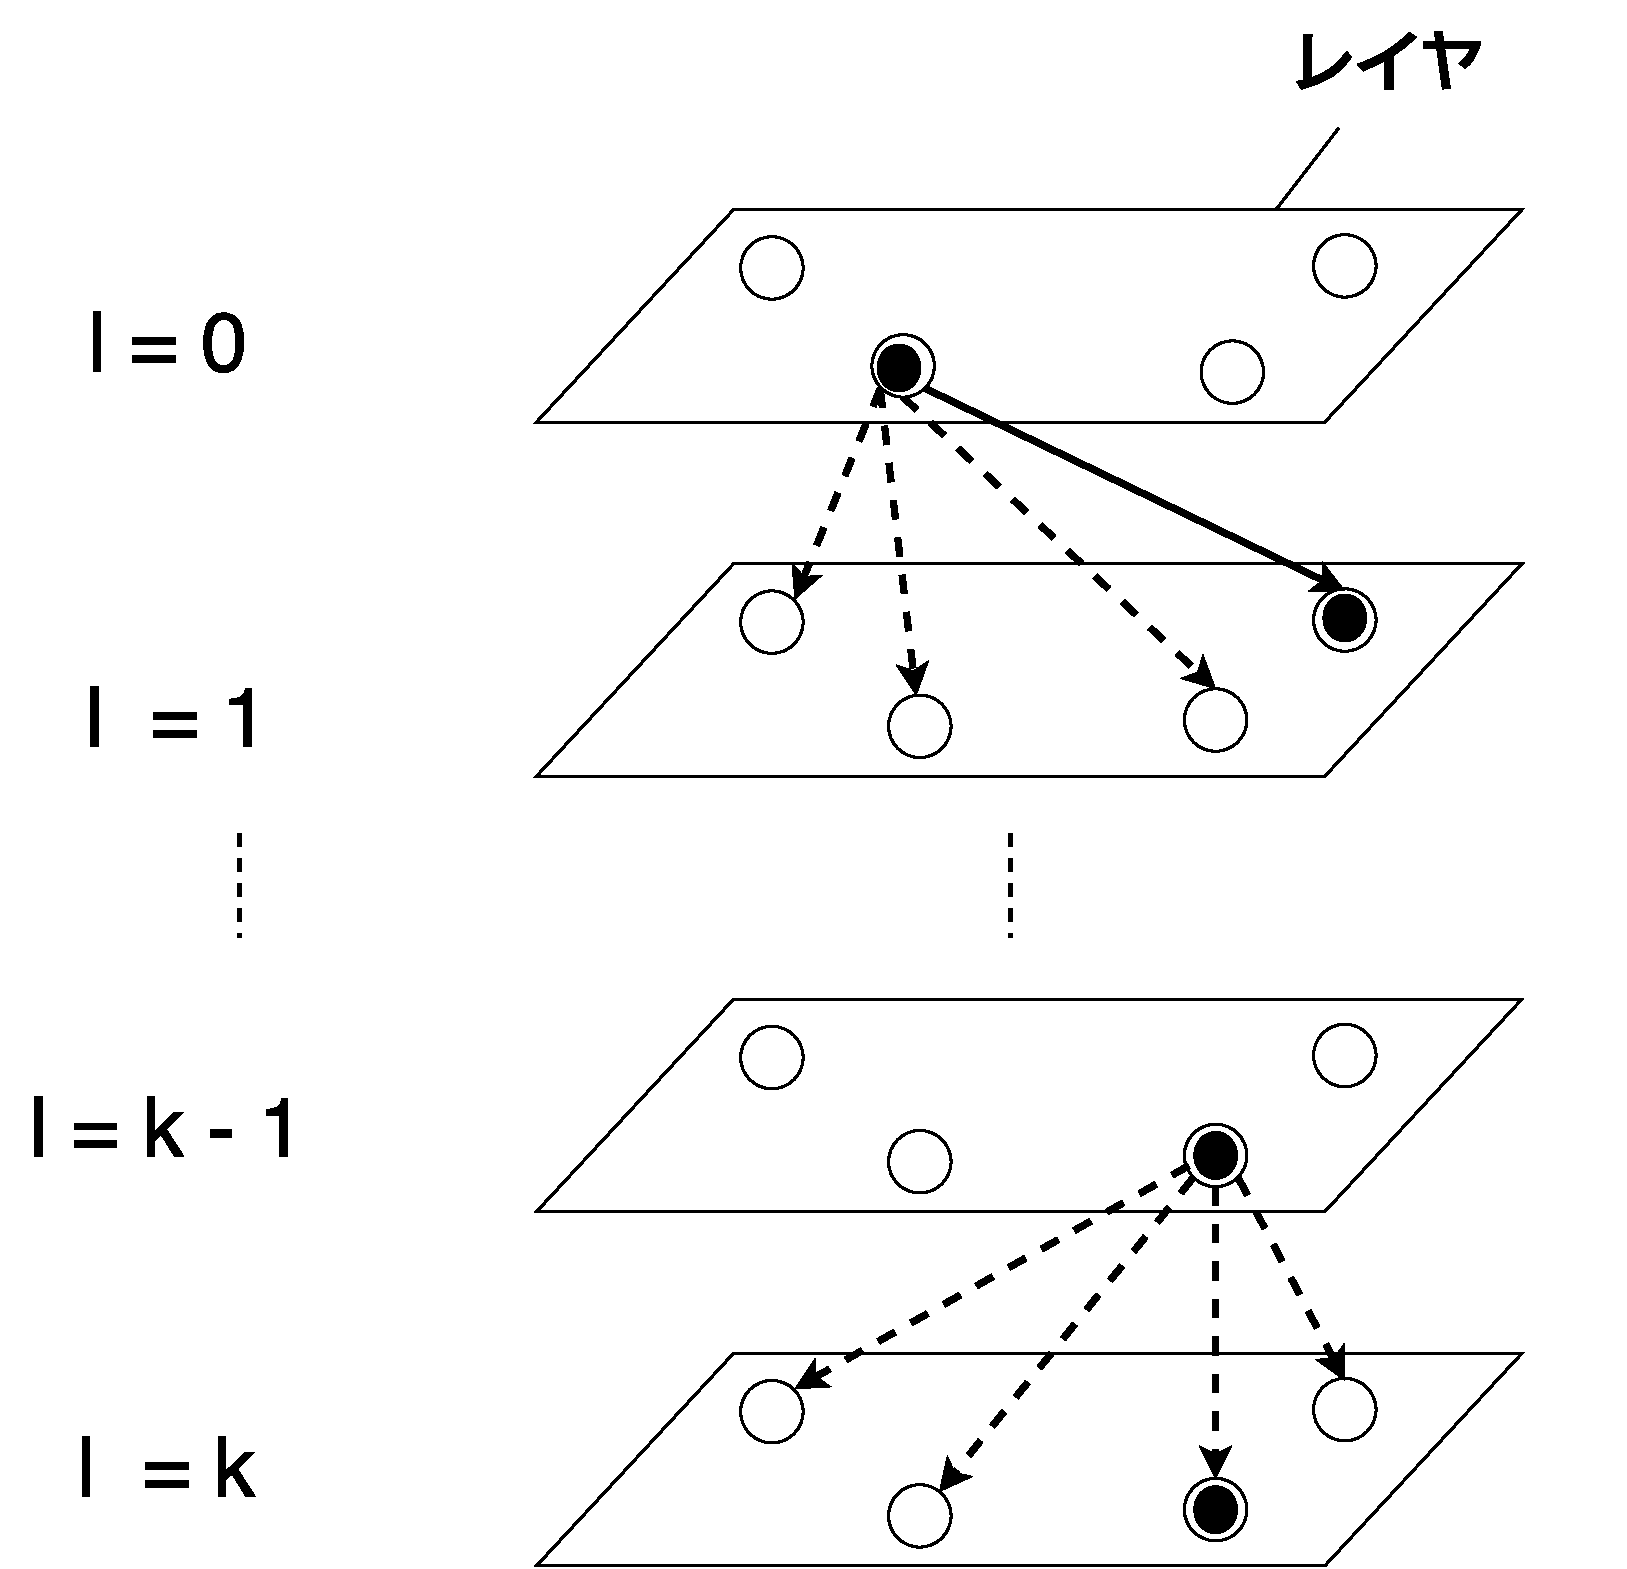
\includegraphics[width=59mm]{./zikuukan_zu.pdf}
    \vspace{-4mm}
    \label{fig:zikuukann}
  \end{figure}
  \begin{itemize}
  \item 各チームの移動回数 $l=0, 1, ..., k$ とし,レイヤと対応させる
  \item 各レイヤ上に出入口を設置し,設置チームが\\どの出入口に移動して止水板を設置するか
  \end{itemize}
} 
%%%%%%%%%%%%%%%%%%%%%%%%%%%%%%%%%%%%%%%%%%%%%%%%%%%%%%%%%%
%%%%%%%%%%%%%%%%%%%%%%%%%%%%%%%%%%%%%%%%%%%%%%%%%%%%%%%%%%%    
\frame{
  \frametitle{最適化問題:定式化}
  \begin{description}
  \item [目的関数]「流入開始時刻に間に合わなかった出入口の止水板設置完了時刻」と「流入開始時刻」の差の合計を最小にする
  \item [制約条件1]初期状態の設定
  \item [制約条件2]流入する全出入口に止水板を設置する
  \item [制約条件3]各設置チームは移動の際に高々 1 つの\\出入口に存在することができる
  \item [制約条件4]枝と節点の関係性
  \item [制約条件5]出入口間の移動時間を求める
  \item [制約条件6]各出入口の流入開始時刻を求める
  \item [制約条件7]止水板設置完了時刻を求める
  \end{description}
}
%%%%%%%%%%%%%%%%%%%%%%%%%%%%%%%%%%%%%%%%%%%%%%%%%%%%%%%
\frame{
  \frametitle{本研究の対象地区}
  \begin{figure}[H]
    \centering
    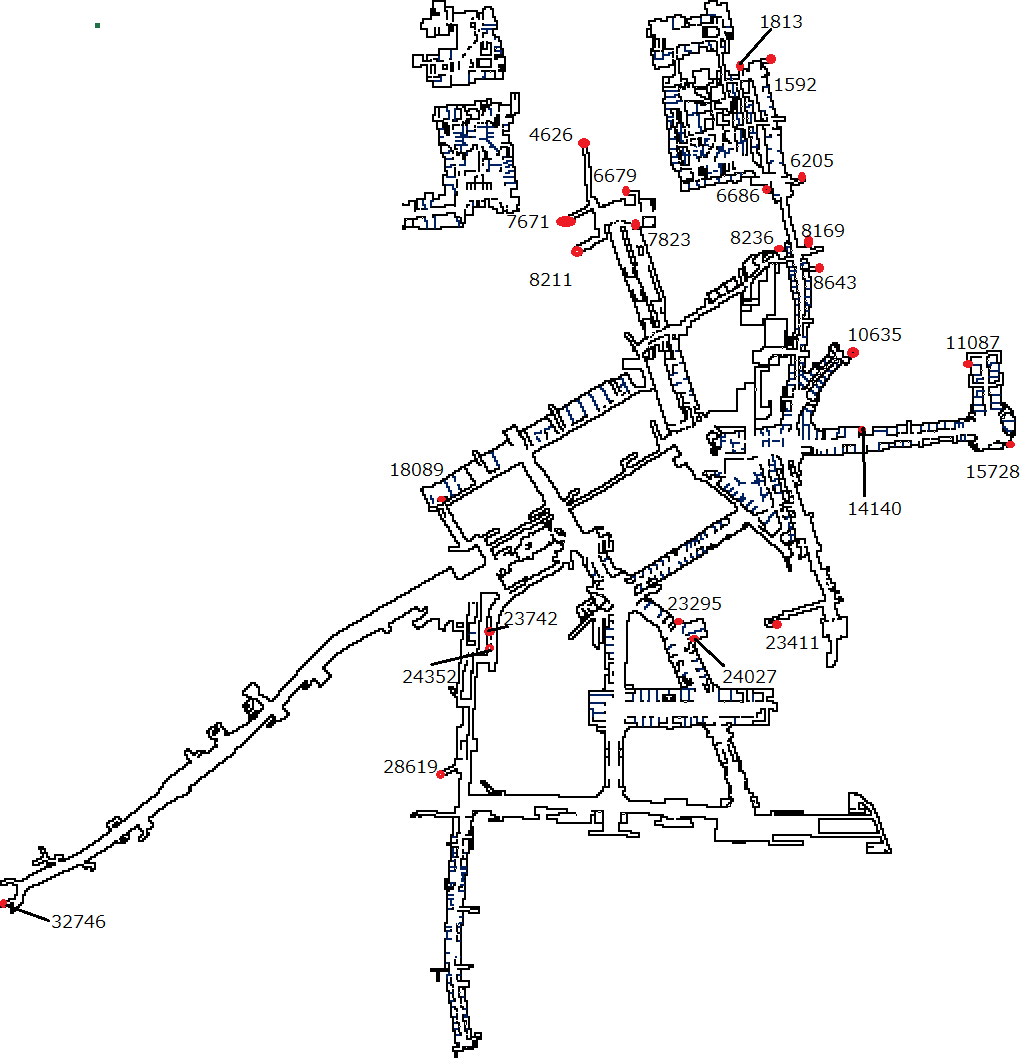
\includegraphics[scale=0.35]{umedamap.png}
  \end{figure}              
}
%%%%%%%%%%%%%%%%%%%%%%%%%%%%%%%%%%%%%%%%%%%%%%%%%%%%%%%
\frame{
  \frametitle{数値実験 実験 1:基本ケース}
  実験 1 では,以下の条件で計算を行った:
  \vspace{-4mm}
  \begin{table}[H]
    \begin{center}
      \begin{tabular}{ll}
        \hline
        1 時間あたりの降雨量 & 60mm \\
        排水用ポンプ & 機能停止 \\
        雨水が流入する出入口の数 & 24 箇所 \\
        止水板設置チーム数 & 6 チーム \\
        止水板設置チームの歩行速度 & 66 m/分  \\
        降雨開始から止水板設置開始までの時間 & 60 分 \\
        止水板 1 箇所の設置に要する時間 & 3 分 \\
        \hline
      \end{tabular}
    \end{center}
  \end{table}
}
%%%%%%%%%%%%%%%%%%%%%%%%%%%%%%%%%%%%%%%%%%%%%%%%%%%%%%%%%%
\frame{
  \frametitle{実験 1 結果:最適設置順序}
  \begin{figure}[H]
    \centering
    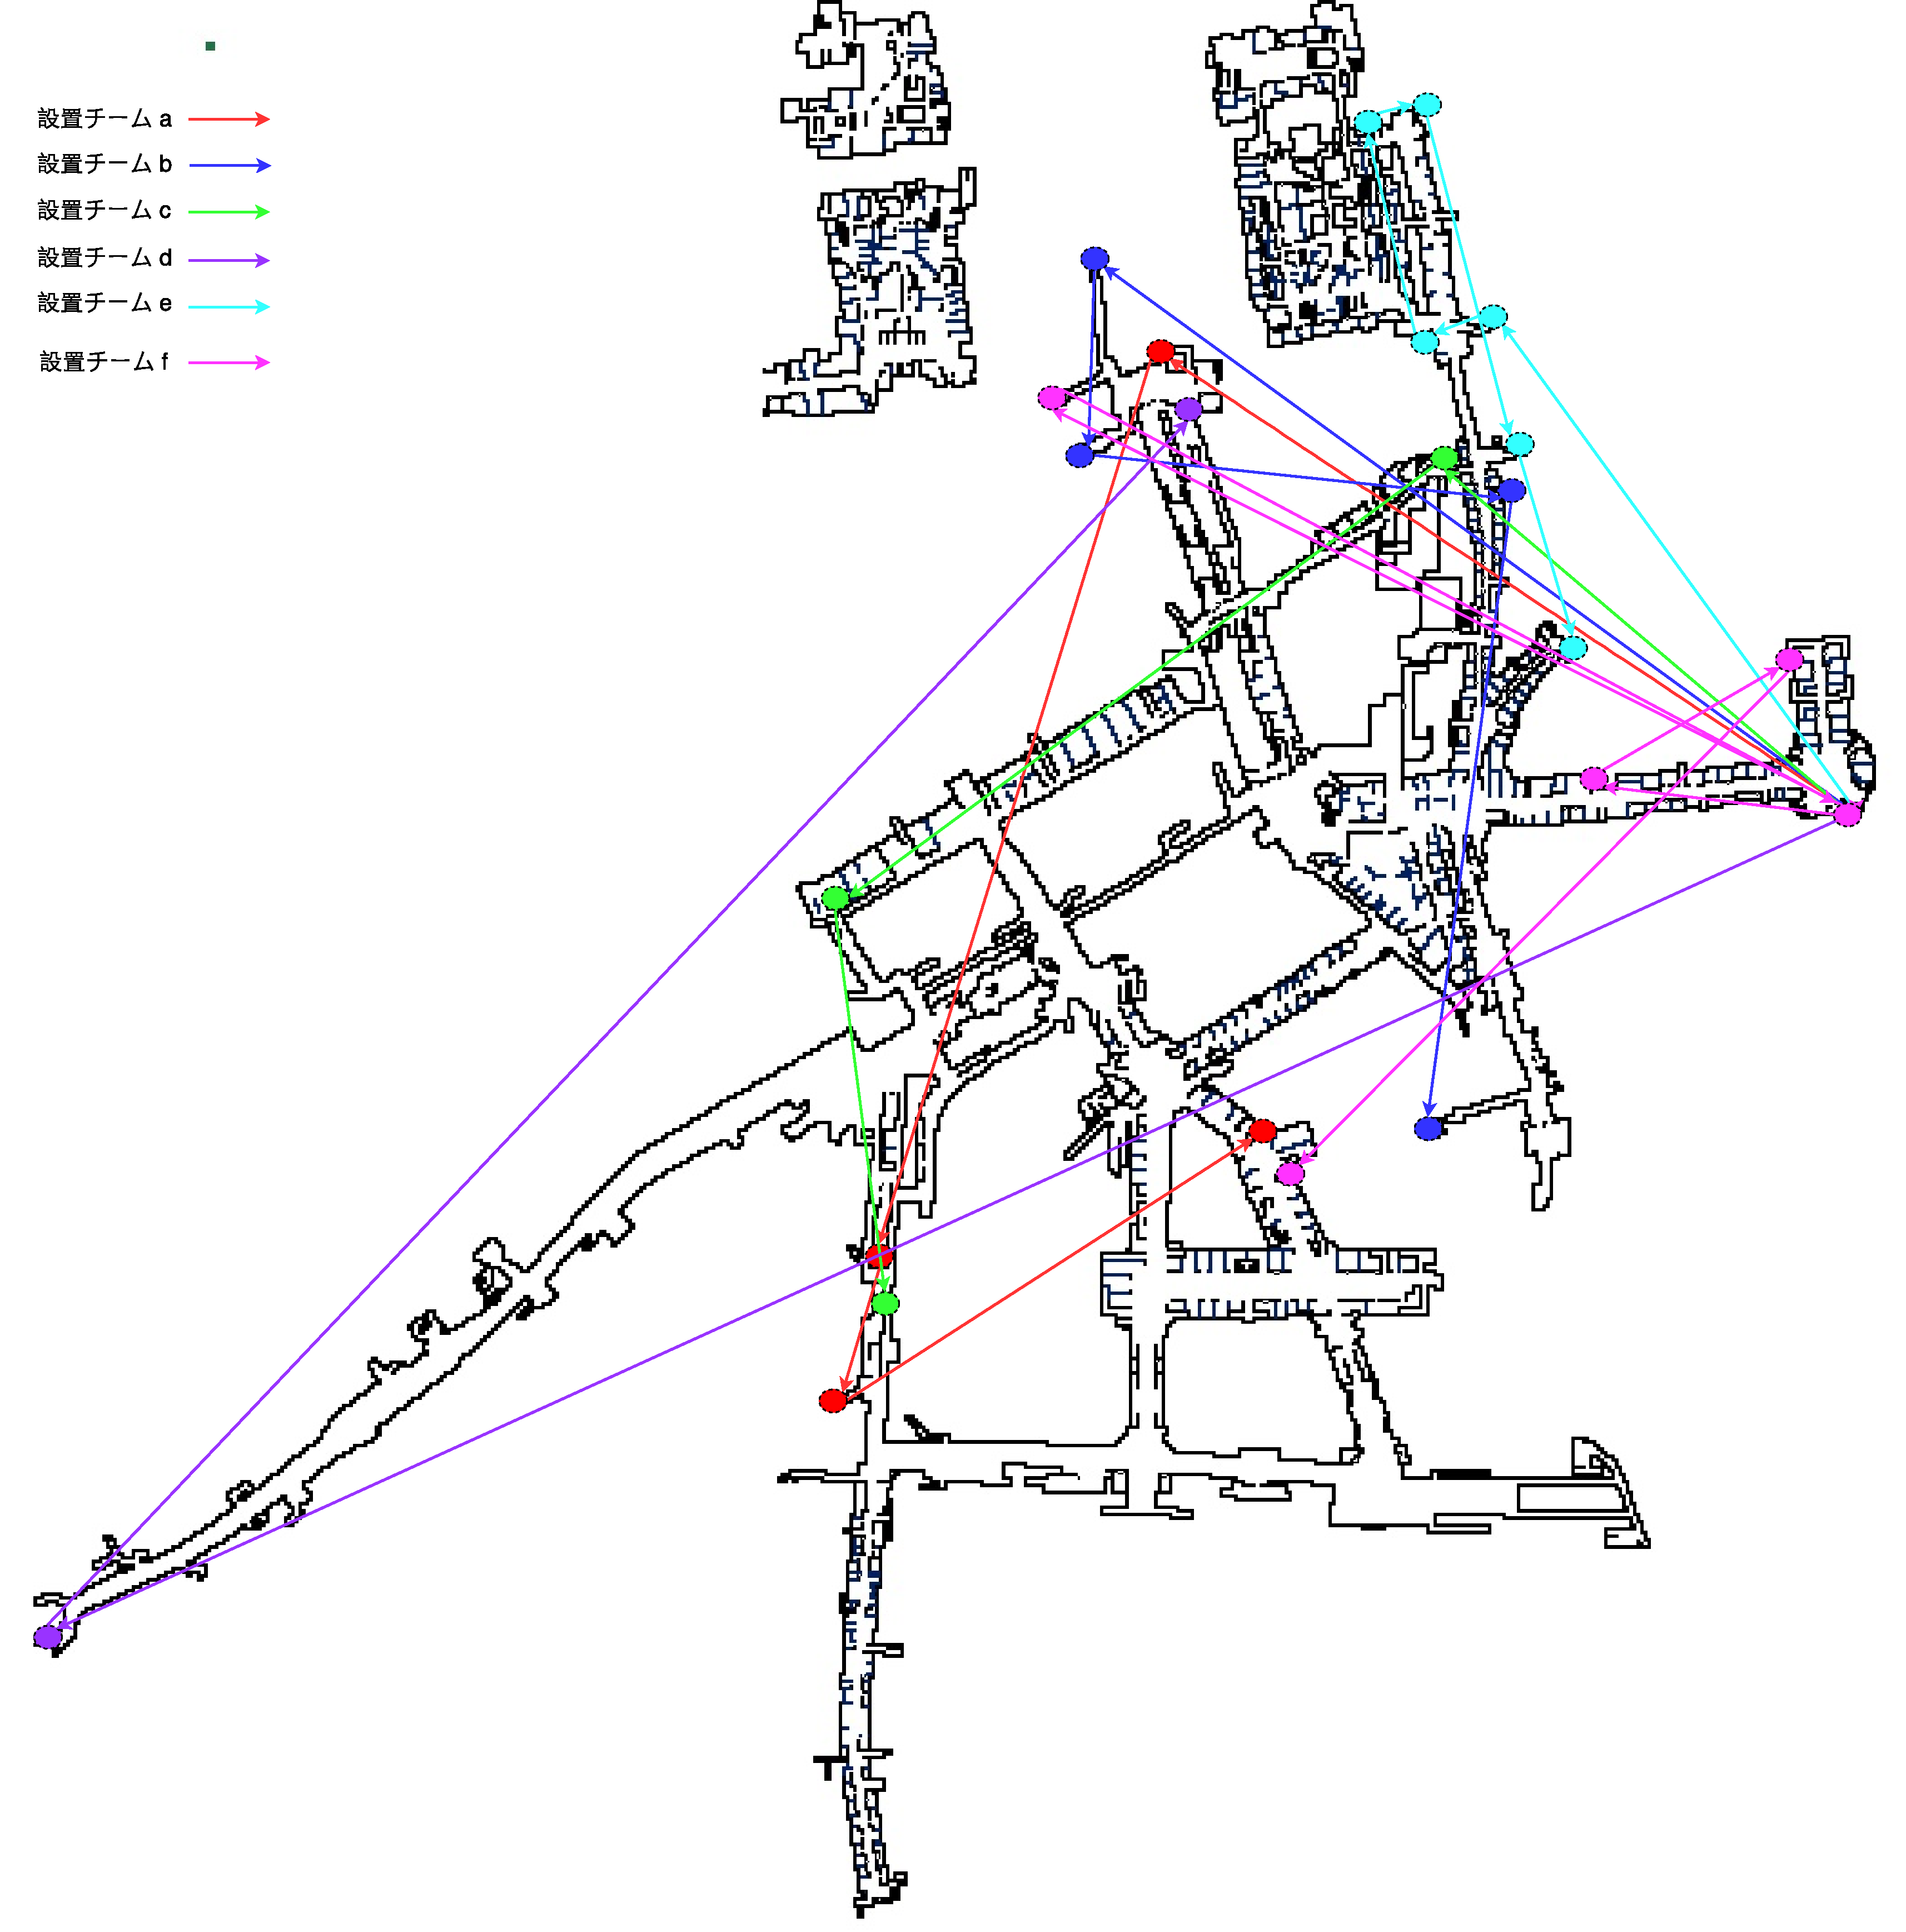
\includegraphics[scale=0.135]{zikken1_settizyunzyo_map.pdf}
  \end{figure}              
}
%%%%%%%%%%%%%%%%%%%%%%%%%%%%%%%%%%%%%%%%%%%%%%%%%%%%%%%%%%%%%%%%%%%%%%%%%%%%
\frame{
  \frametitle{実験 1 結果:各出入口への設置状況}
  \begin{figure}[H]
    \centering
    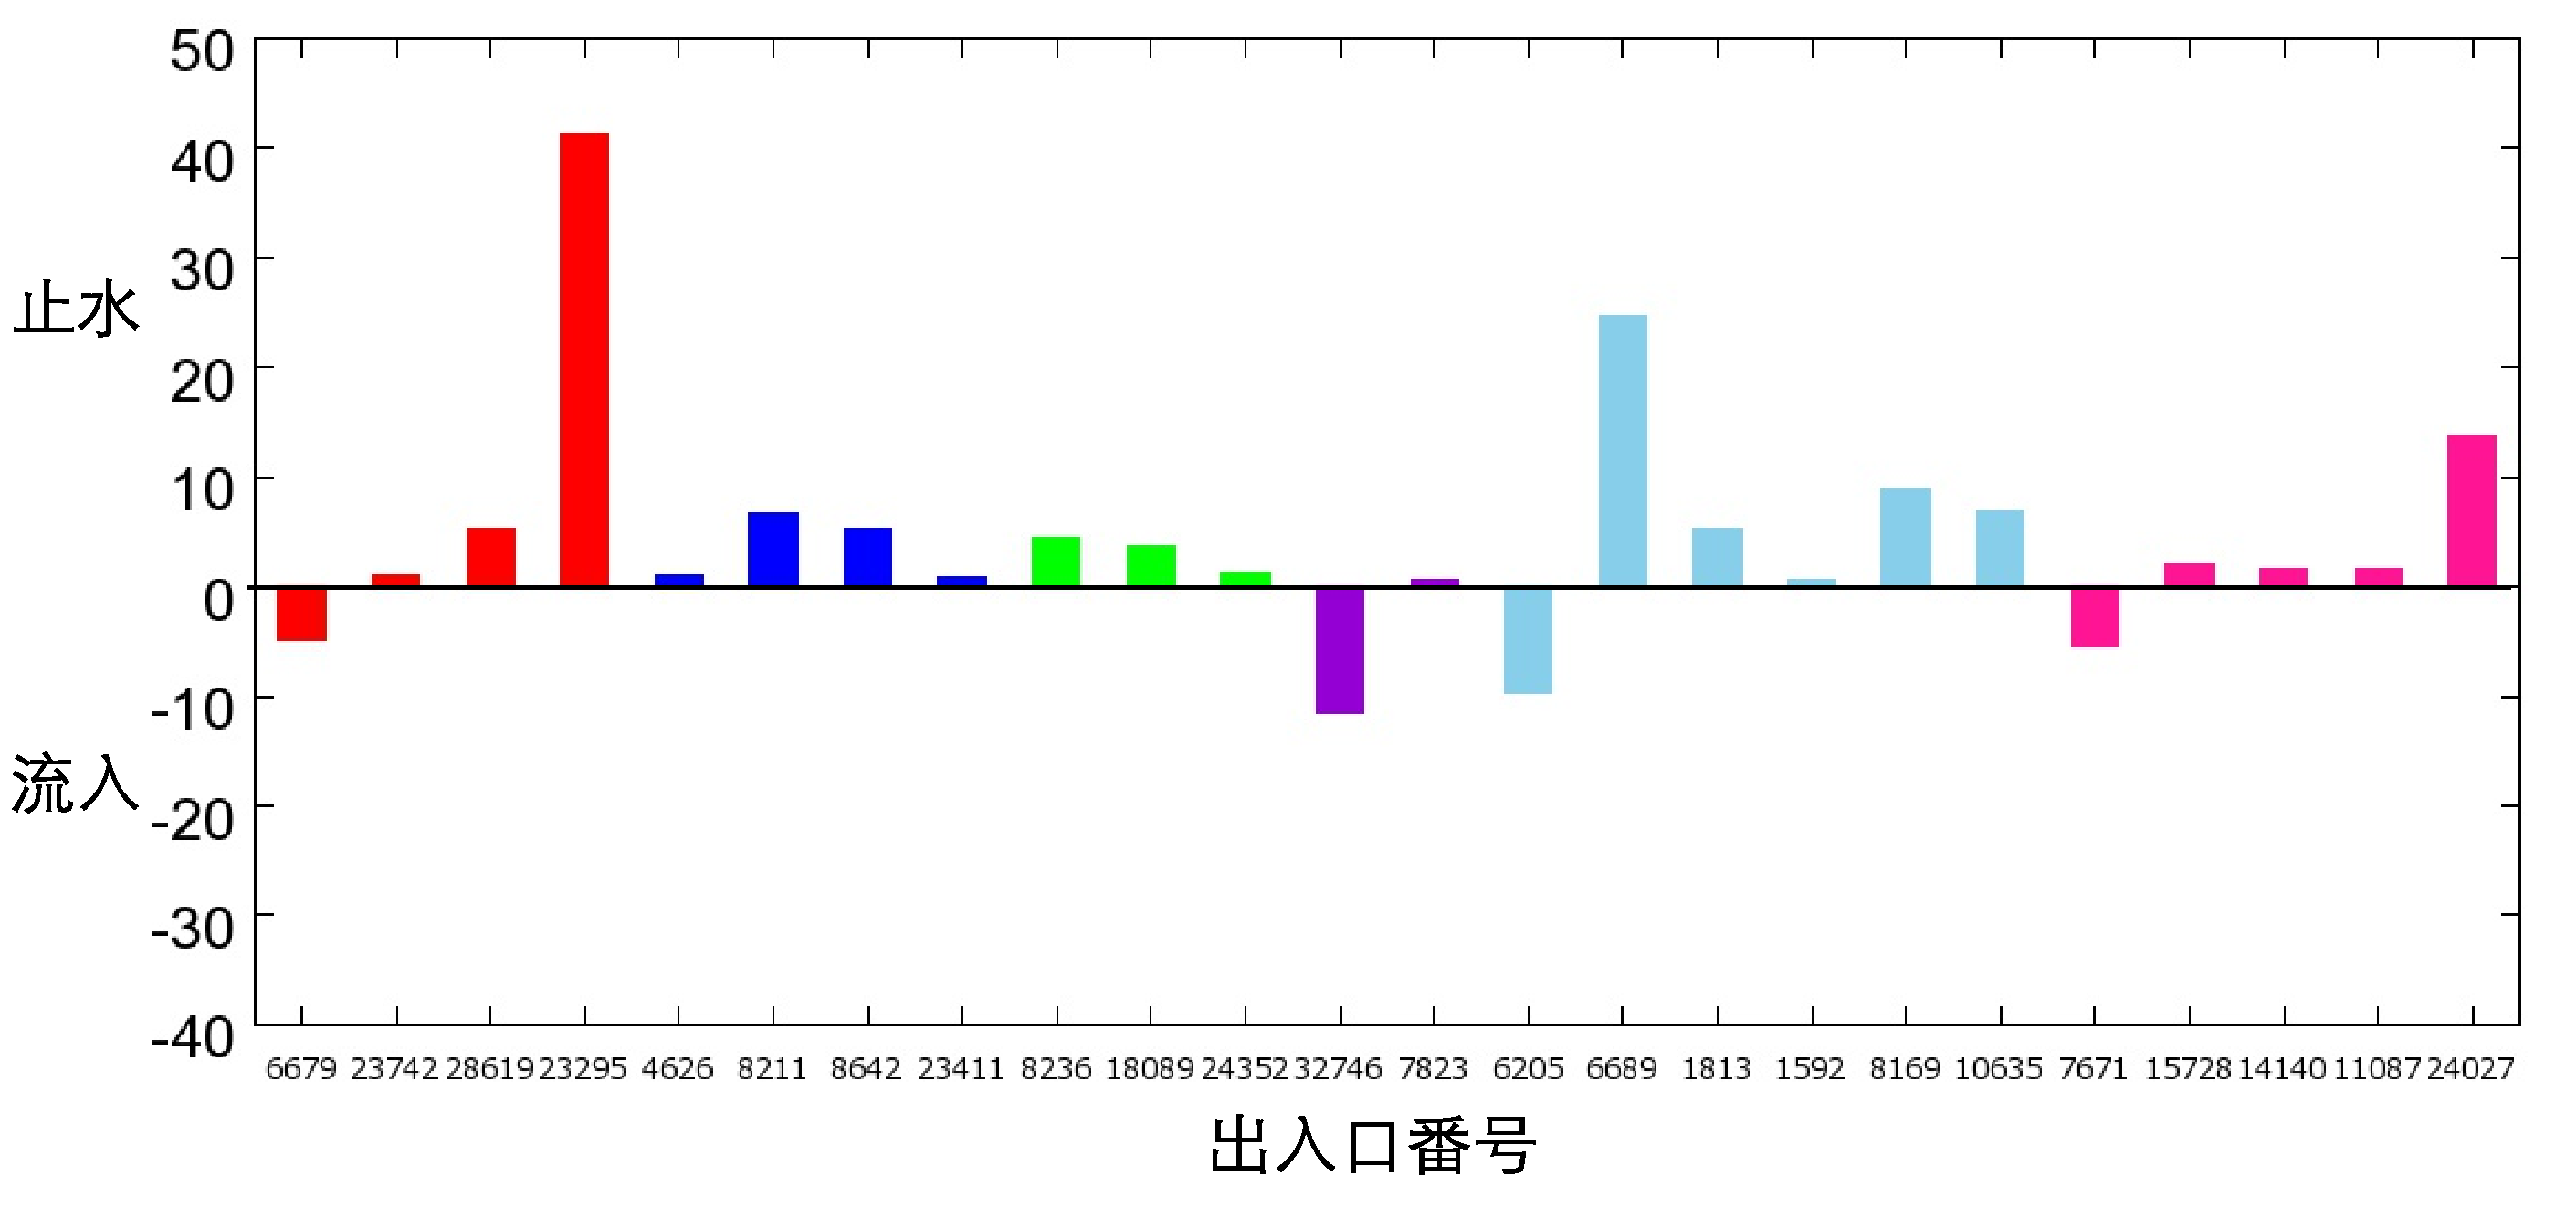
\includegraphics[scale=0.26]{zikken1_gurahu.pdf}
    \caption{各出入口への設置状況(実験 1:6 チーム)}
  \end{figure}              
}
%%%%%%%%%%%%%%%%%%%%%%%%%%%%%%%%%%%%%%%%%%%%%%%%%%%%%%%%%%
\frame{
\begin{figure}[H]
    \centering
    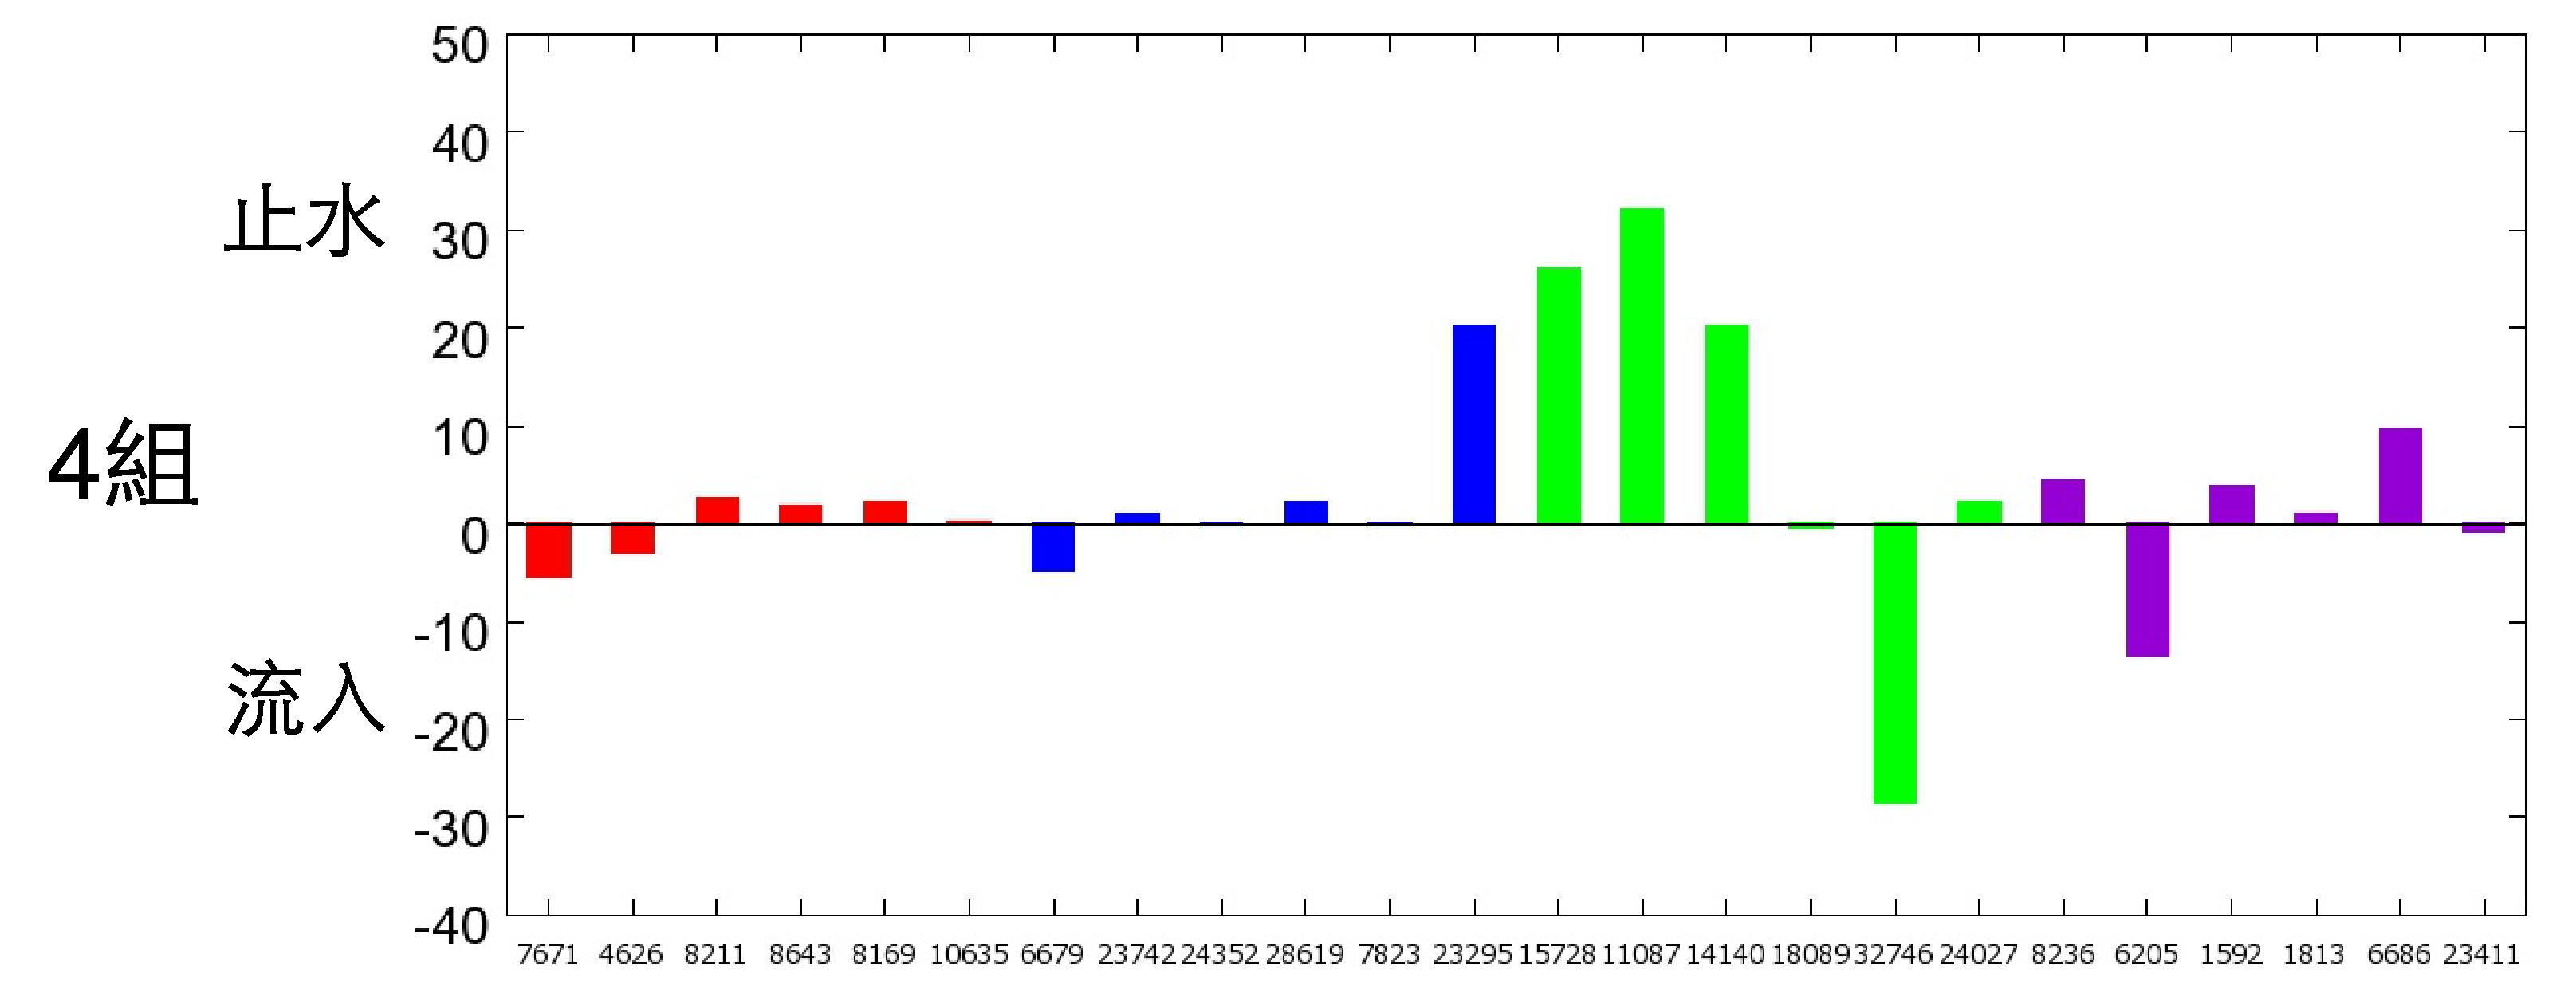
\includegraphics[height=20mm,width=90mm]{zikken2_4team_gurahu.pdf}
  \end{figure}              
\begin{figure}[H]
  \vspace{-2mm}
    \centering
    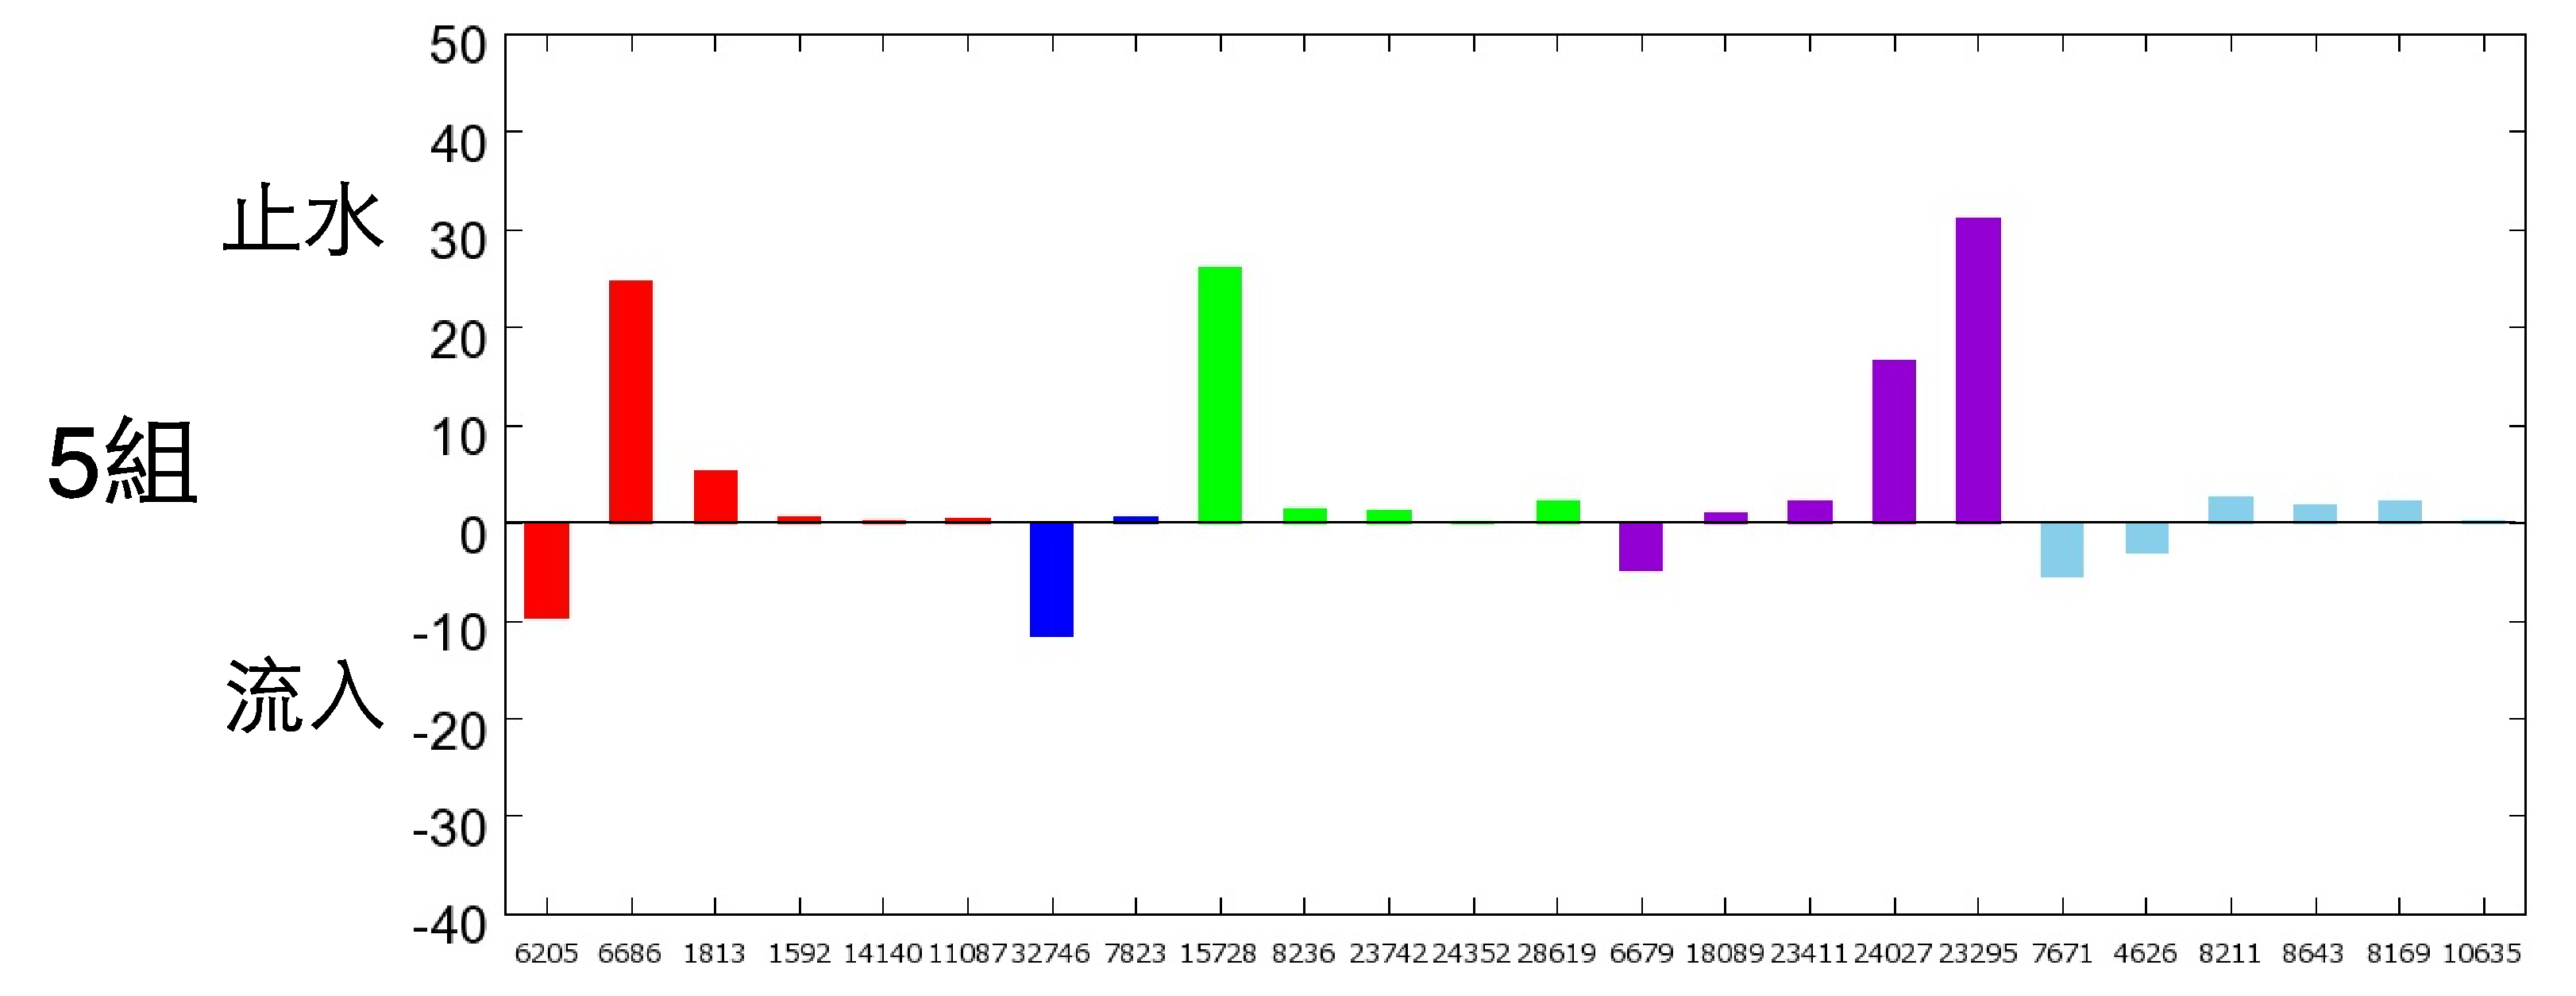
\includegraphics[height=20mm,width=90mm]{zikken2_5team_gurahu.pdf}
  \end{figure}
\begin{figure}[H]
  \vspace{-2mm}
    \centering
    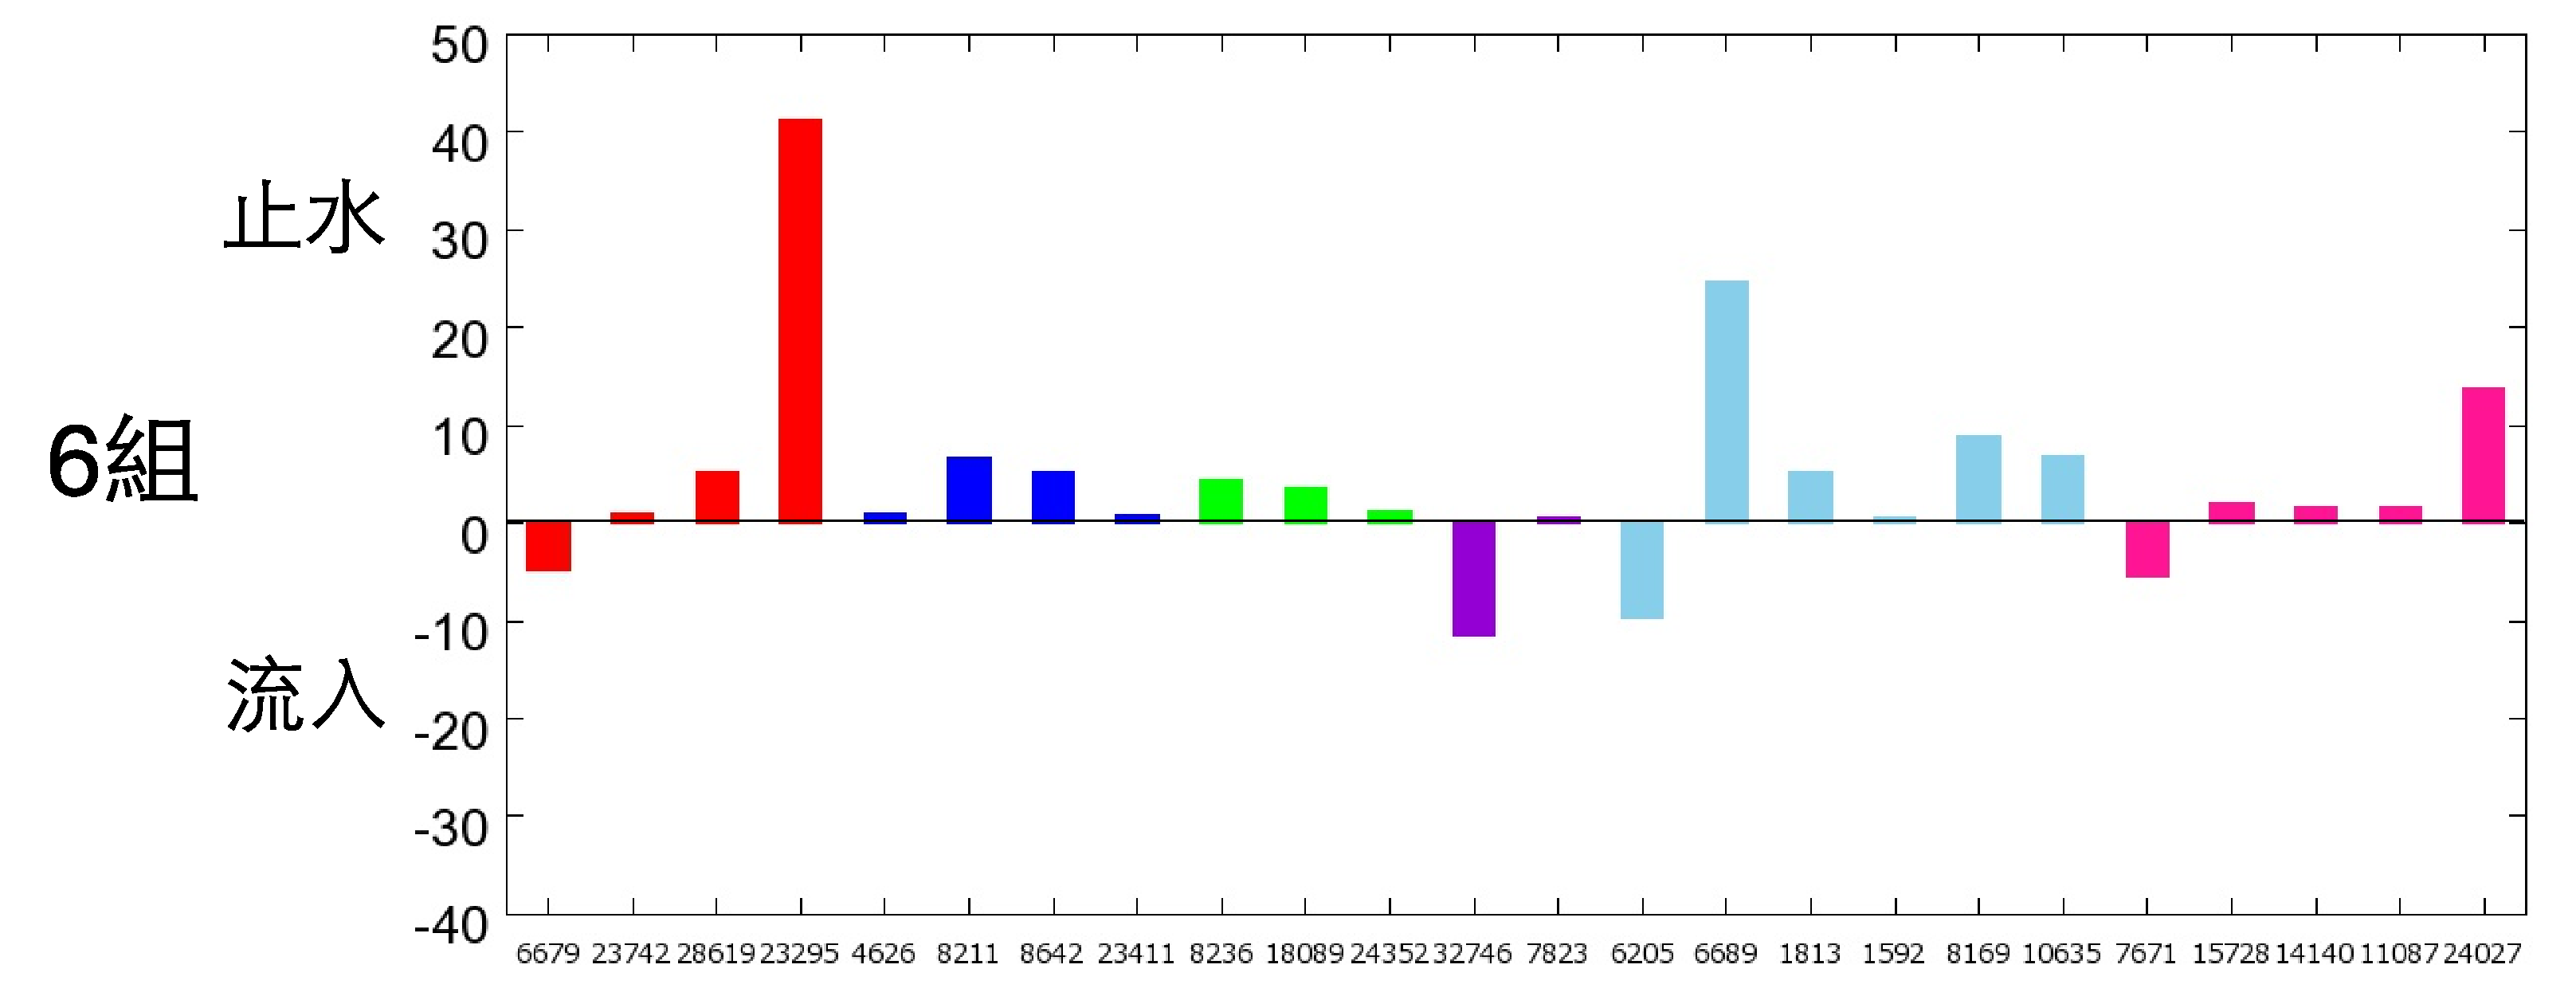
\includegraphics[height=20mm,width=90mm]{zikken2_6team_gurahu.pdf}
  \end{figure}              
\begin{figure}[H]
  \vspace{-2mm}
    \centering
    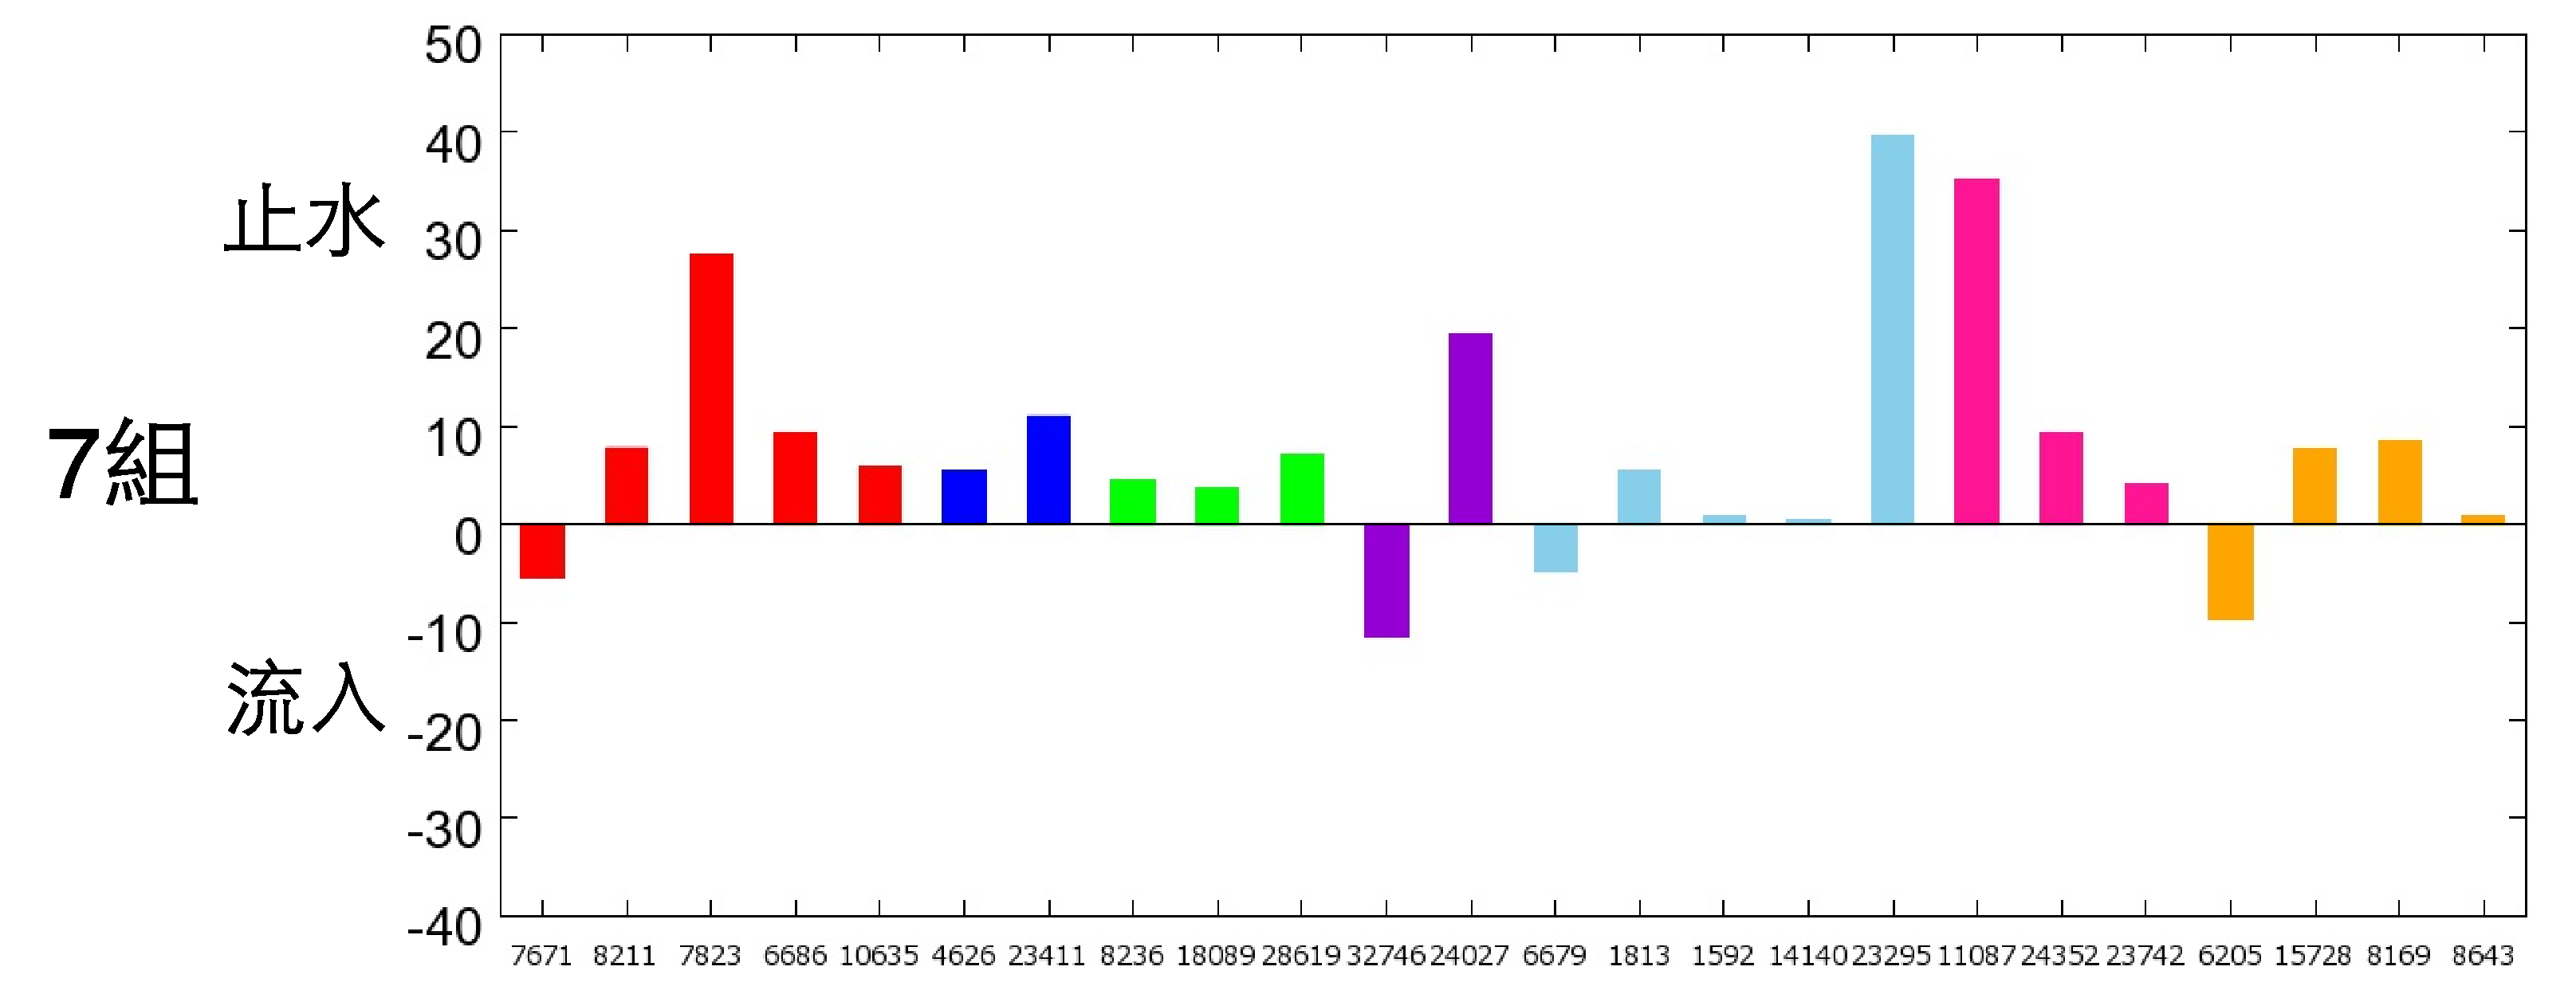
\includegraphics[height=20mm,width=90mm]{zikken2_7team_gurahu.pdf}
  \end{figure}              
    }
%%%%%%%%%%%%%%%%%%%%%%%%%%%%%%%%%%%%%%%%%%%%%%%%%%%%%%%%%%
\begin{comment}
%%%%%%%%%%%%%%%%%%%%%%%%%%%%%%%%%%%%%%%%%%%%%%%%%%%%%%%%%
\frame{
  \frametitle{実験 2:設置条件の比較(1/3)}
  実験 1 の設置チームの数を 4組,5組,7組に変更
  \begin{figure}[H]
    \centering
    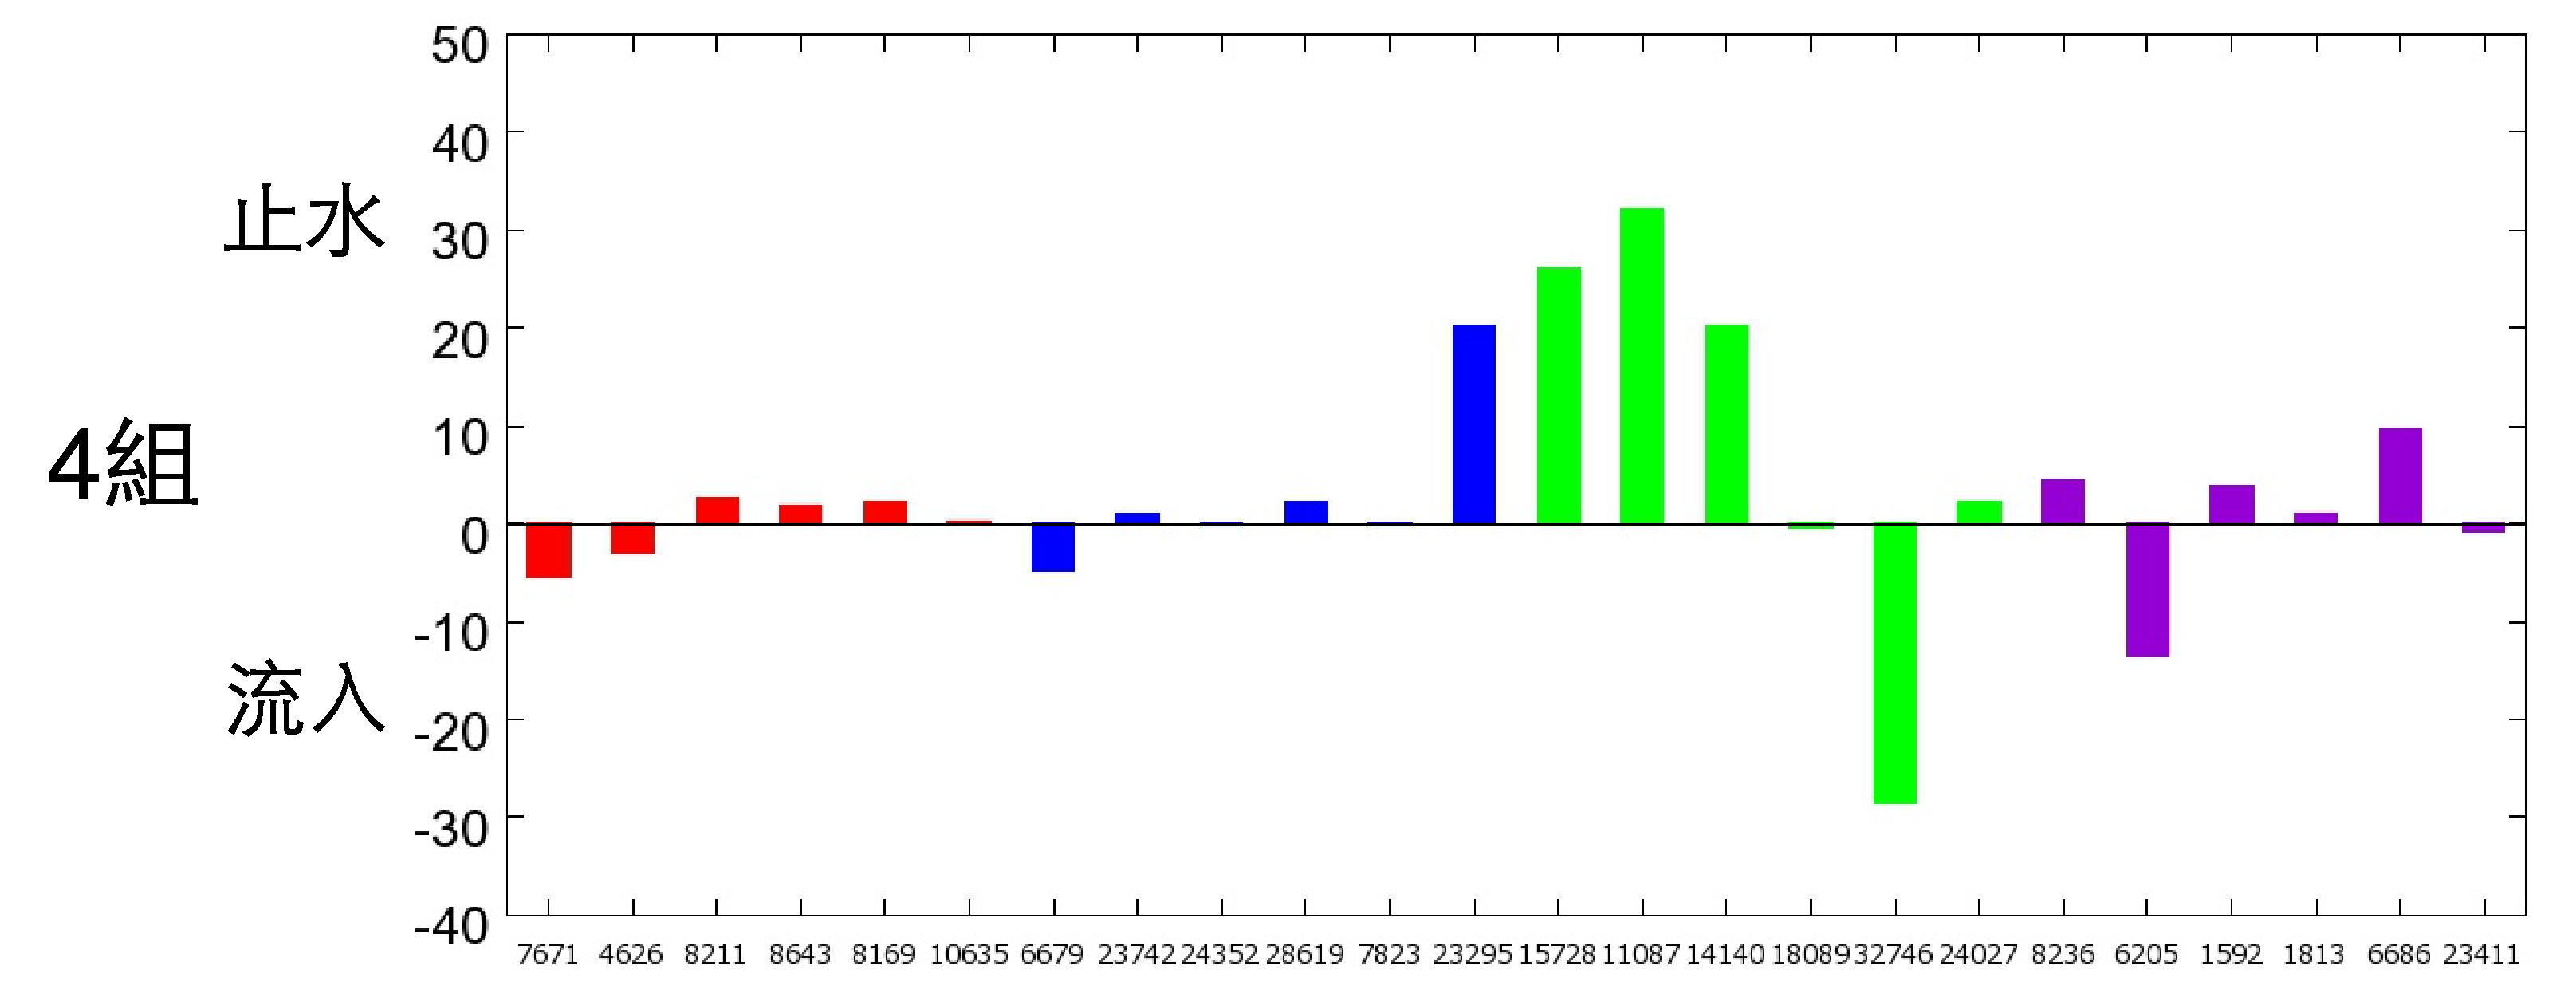
\includegraphics[scale=0.26]{zikken2_4team_gurahu.pdf}
    \caption{各出入口への設置状況(実験 2 / 4 チーム)}
  \end{figure}              
}
%%%%%%%%%%%%%%%%%%%%%%%%%%%%%%%%%%%%%%%%%%%%%%%%%%%%%%%
\frame{
  \frametitle{実験 2:設置条件の比較(2/3)}
  \begin{figure}[H]
    \centering
    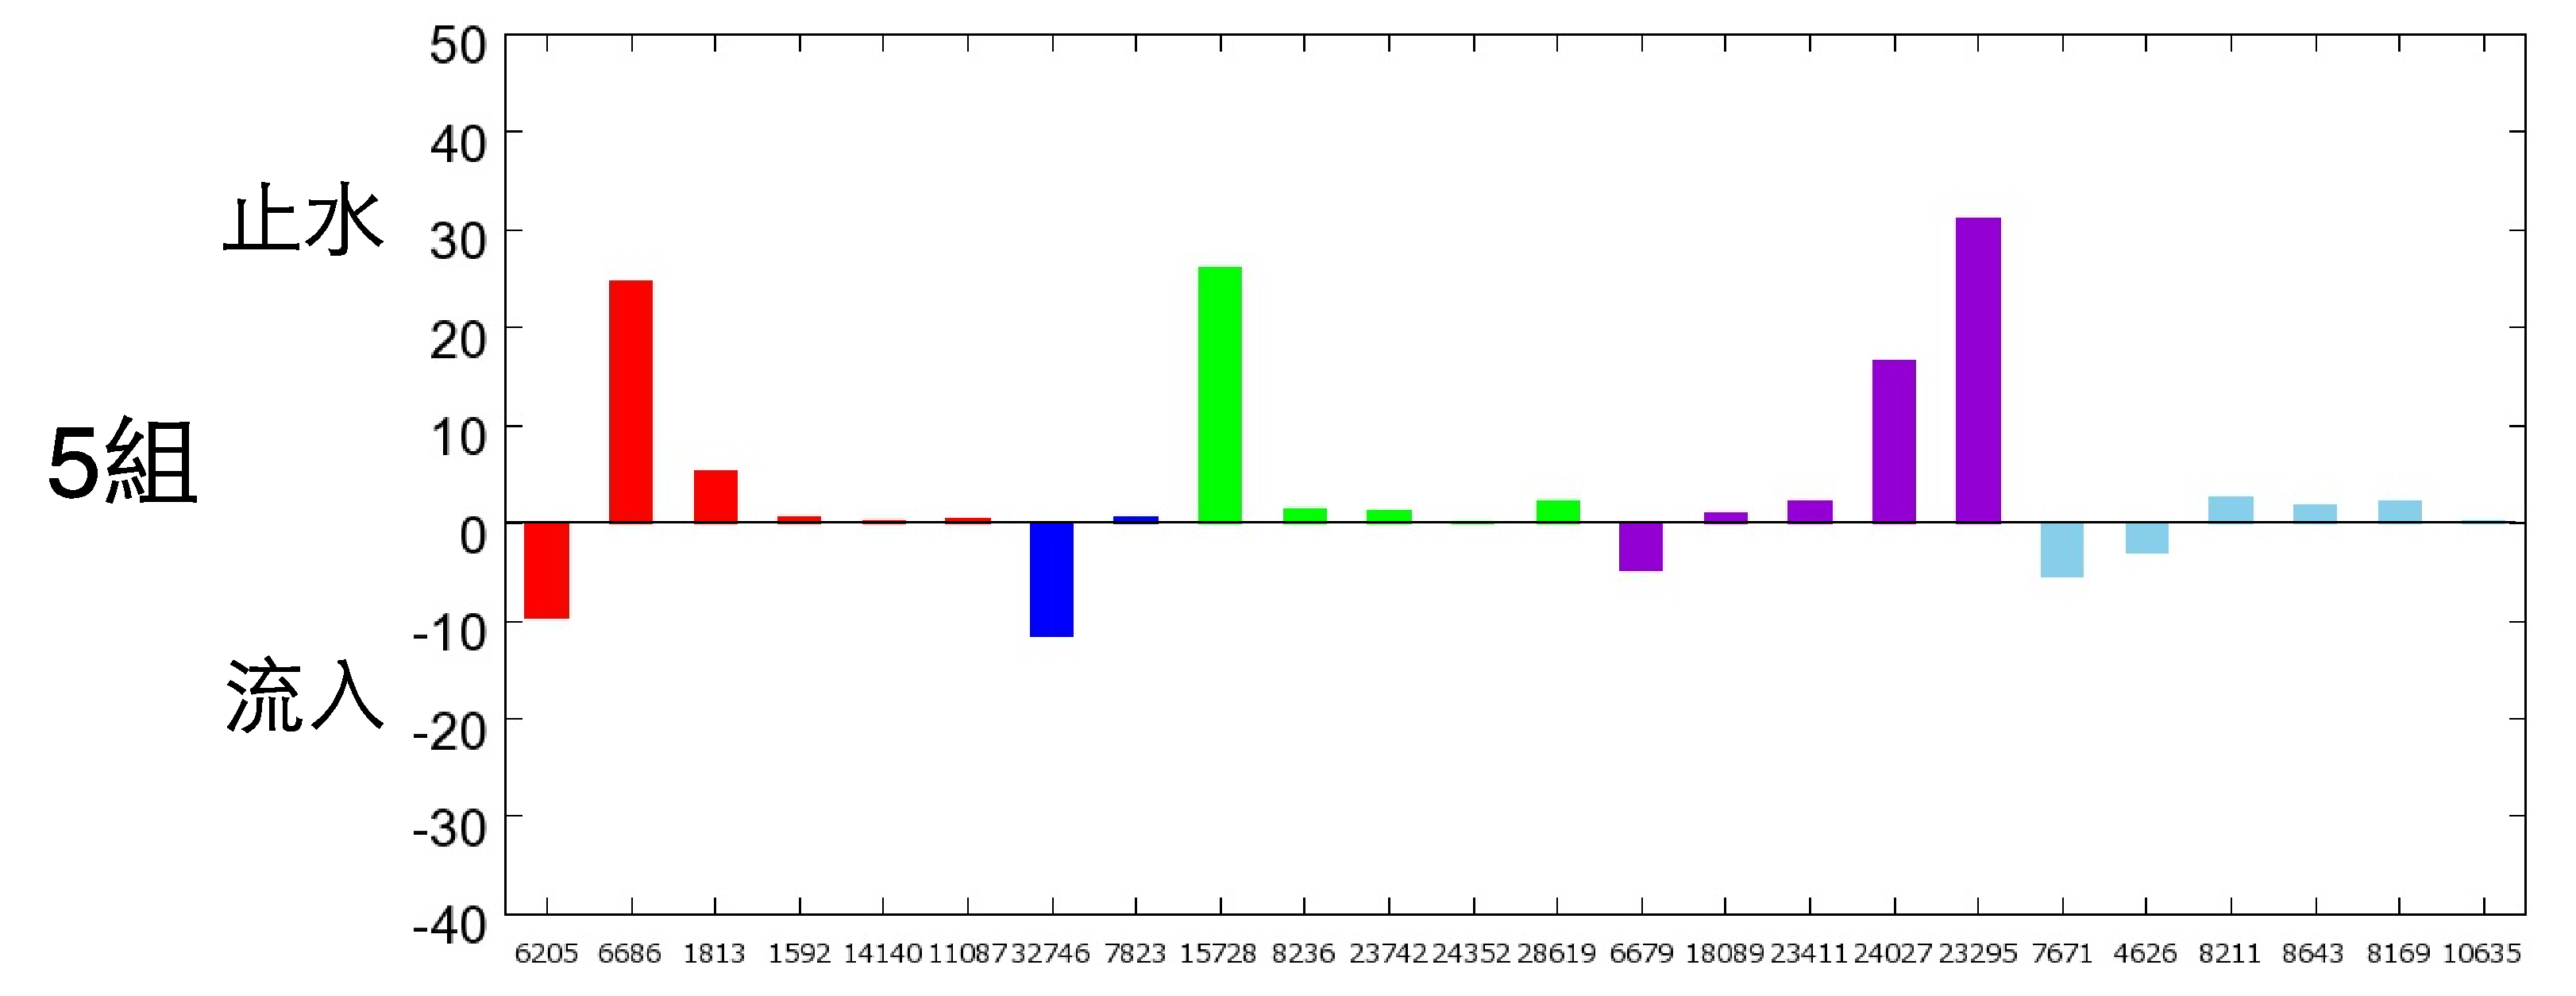
\includegraphics[scale=0.26]{zikken2_5team_gurahu.pdf}
    \caption{各出入口への設置状況(実験 2 / 5 チーム)}
  \end{figure}              
}
%%%%%%%%%%%%%%%%%%%%%%%%%%%%%%%%%%%%%%%%%%%%%%%%%%%%%%%%%%
\frame{
  \frametitle{実験 2:設置条件の比較(3/3)}
  \begin{figure}[H]
    \centering
    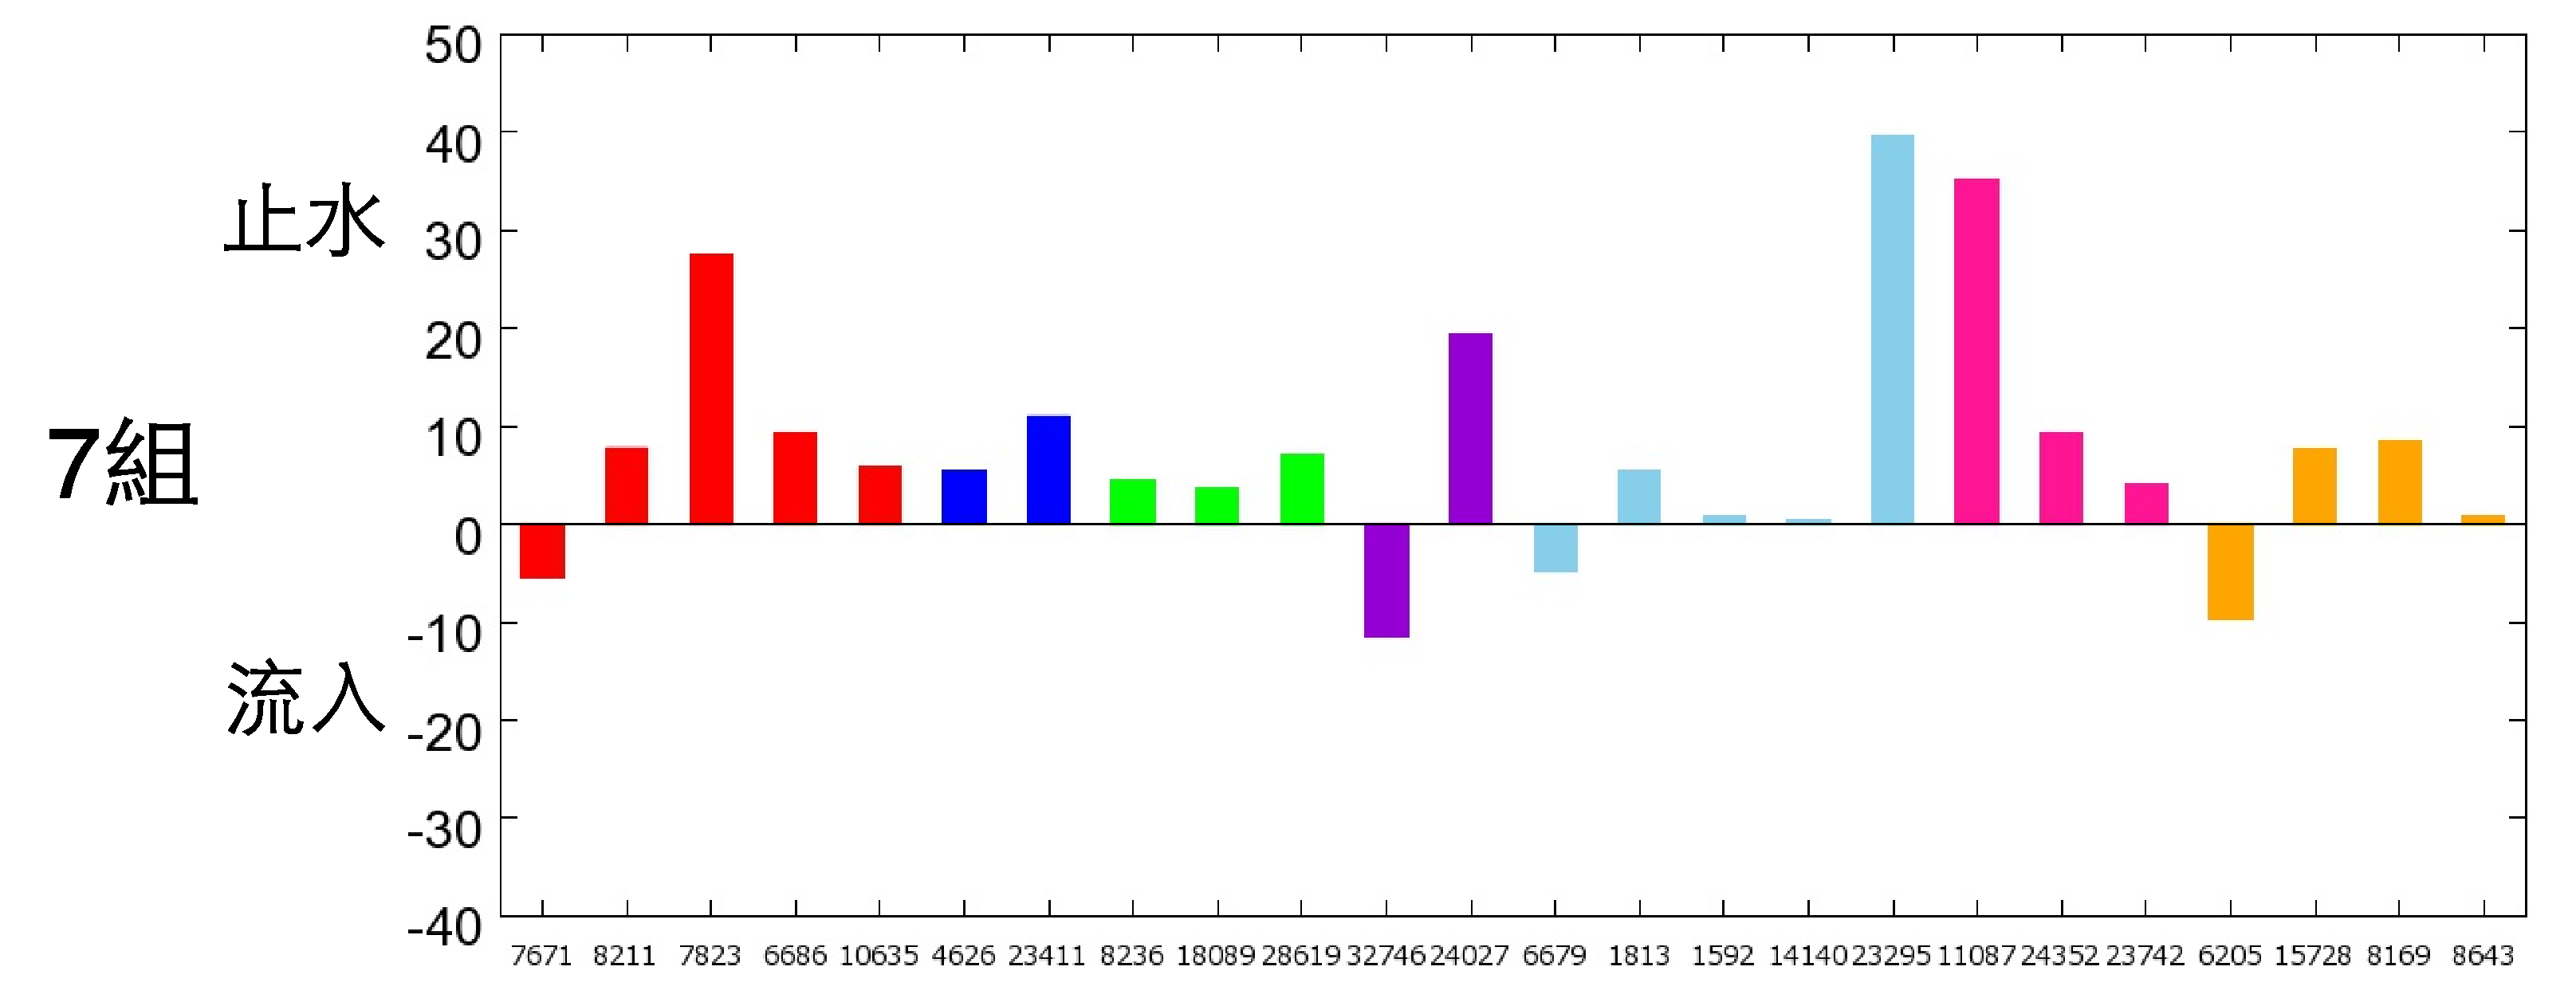
\includegraphics[scale=0.26]{zikken2_7team_gurahu.pdf}
    \caption{各出入口への設置状況(実験 2 / 7 チーム)}
  \end{figure}              
}
%%%%%%%%%%%%%%%%%%%%%%%%%%%%%%%%%%%%%%%%%%%%%%%%%%%%%%%%%%%%
\end{comment}
%%%%%%%%%%%%%%%%%%%%%%%%%%%%%%%%%%%%%%%%%%%%%%%%%%%%%%%%%%
\frame{
  \frametitle{実験結果まとめ }
  \begin{itemize}
  \item 計算時間の上限は 86400 秒 (=24 時間)
    \begin{itemize}
    \item 86400秒以上の時間がかかる場合は暫定解を表示
    \end{itemize}
  \end{itemize}
  \begin{tabular}{lrrr}
    \hline
    チーム数 & 計算時間(秒) &  流入時間の合計(分) \\
    \hline
    4     &  86400 & 57.06\\
    5     &  59610 & 34.55\\
    6     &  20875 & 31.36\\
    7     &  1446  & 31.36\\
    \hline
  \end{tabular}
  \begin{beamerboxesrounded}
    {}
    止水板設置チームの数が増えるほど地下街に流入する\\時間は短くなっているが,チーム数が一定の数まで\\増えると地下街に流入する時間は変化がなくなる.
  \end{beamerboxesrounded}                                                        
}
%%%%%%%%%%%%%%%%%%%%%%%%%%%%%%%%%%%%%%%%%%%%%%%%%%%%%%%%%%

%%%%%%%%%%%%%%%%%%%%%%%%%%%%%%%%%%%%%%%%%%%%%%%%%%%%%%%%%%
\frame{
  \frametitle{おわりに}
  \begin{beamerboxesrounded}
    {まとめ}
    \begin{itemize}
    \item 各出入口の流入開始時刻を考慮した最適な\\止水板の設置順序を算出することができた
    \item 止水板の設置条件を変えることで条件の比較を\\行うことができた
    \end{itemize}
  \end{beamerboxesrounded}
  \begin{beamerboxesrounded}
    {今後の検討課題}
    \begin{itemize}
    \item 1 時間あたりの降雨量を増やした場合,流入する出入口の数が増え,その結果,計算時間が\\大幅に長くなる\\
      $\Rightarrow$ 新たな最適化モデルの構築が必要
    \end{itemize}
  \end{beamerboxesrounded}
}
%%%%%%%%%%%%%%%%%%%%%%%%%%%%%%%%%%%%%%%%%%%%%%%%%%%%%%
\end{document}
